\begin{figure}[t]\label{ex:pow_block}
       \centering
   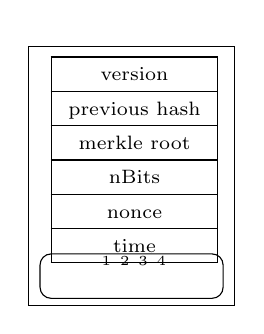
\begin{tikzpicture}[yscale=0.47,xscale=0.75]
   	\draw (0,0) rectangle (3.5,7);
   	\draw[rounded corners] (0.2,0.2) rectangle (3.3,1.4);
   	
   	\node[label,below] at(1.8,1.6) {\scriptsize $\Transaction_1$ $\Transaction_2$ $\Transaction_3$ $\Transaction_4$};
   	\node[label,below] at(1.8,7) {
	\begin{tabular}{|c|c|} \hline
              {\scriptsize \MName{version}}   		\\ \hline
	      {\scriptsize \MName{previous hash}} 	\\ \hline
              {\scriptsize \MName{merkle root}}  	\\ \hline
              {\scriptsize \MName{nBits}} 		\\ \hline
              {\scriptsize \MName{nonce}} 		\\ \hline
              {\scriptsize \MName{time}}  		\\ \hline
	\end{tabular}
	};
 
   \end{tikzpicture}
   \caption{A Bitcoin-style block containing a header and a body with transactions ($\Transaction_1$, $\Transaction_2$, $\Transaction_3$ and $\Transaction_4$).}
   \label{fig:block-structure}
\end{figure}

\section{Background: Proof-of-Work Consensus}
The {\em settlement} phase in our \DualChain{} architecture makes use of 
our novel \PoC{} protocol. The intuition behind \PoC's design stems from the 
\PoW{} protocol that helps create an immutable {\em chain of blocks}. The term 
immutable refers to the fact that each block appended to the chain requires miners 
to spend their resources. As a result, if an adversary attempts to over-write 
(or rollback) a part of the chain, it needs to create an alternate chain of all the 
desired blocks. However, to force all the honest miners to switch to this alternate 
chain, the adversary needs to compute this chain of blocks at a much faster rate 
than the original chain. This implies that the adversary needs to have much greater 
power than the honest miners. Prior works have illustrated that such an attack is 
hard to realize~\cite{bc-processing}.

Prior to running the \PoW{} protocol, each miner $\Miner \in \Miners$ needs to 
create a {\em block} of transactions. Although each miner $\Miner$ has access to the 
certificate $\Certificate$, it needs to arrange the contents of this certificate in 
the format of a block. To explain the format of a block, we follow the popular 
blockchain platform, Bitcoin, where each block includes a header and body 
(refer to Figure~\ref{fig:block-structure})~\cite{blockchain-book}. 
The header includes: 
(i) {\em version} for this block, 
(ii) {\em hash} of the previous block, 
(iii) {\em merkle root} of all transactions, 
(iv) {\em nBits}, which determines the difficulty of the puzzle, 
(v) {\em nonce}, the solution for puzzle, and 
(vi) {\em time} at which block is created once the nonce is found.

Computing Merkle root of all the transactions is trivial (refer to 
Figure~\ref{fig:merkle-tree}) and requires a miner $\Miner$ to compute a pairwise 
hash from the leaf to the root. This Merkle root helps to verify if a transaction 
was included to create the Merkle tree. However, the main challenge for a miner is 
to determine the nonce. In existing \PoW{}-based platforms, to solve the complex 
puzzle, each miner needs to calculate the {\em hash of the block} such that it 
contains a specific number of leading zero bits. For this purpose, the miners have 
to find a {\em nonce} value that yields the specific hash. This essentially makes the 
\PoW{} protocol like a {\em race} where all the miners are competing against each 
other to find the nonce. Whichever miner finds a valid nonce first, it gets the chance 
to propose the next block to be added to the chain. Hence, coming up with the correct 
number of leading zero bits in the hash is important as it sets the difficulty of 
the puzzle which simplicity controls the average time taken for each winning miner 
to propose a block. Once a miner finds the valid nonce, it can fill all the entries 
in the header, and it broadcasts the new block to all the other miners.


\begin{figure}[t]\label{ex:merkle_tree}
       \centering
       \begin{tikzpicture}[scale=0.625,transform shape]
           \node[dot] (n1) at (0, 0) {};
           \node[dot] (n2) at (4, 0) {};
           \node[dot] (n3) at (8, 0) {};
           \node[dot] (n4) at (12, 0) {};
           
           \node[below] at (n1) {$h_0 = \Digest{\Transaction_1}$};
           \node[below] at (n2) {$h_1 = \Digest{\Transaction_2}$};
           \node[below] at (n3) {$h_2 = \Digest{\Transaction_3}$};
           \node[below] at (n4) {$h_3 = \Digest{\Transaction_4}$};
   
           \node[dot] (n12) at (2, 1) {} edge[->] (n1) edge[->] (n2);
           \node[dot] (n34) at (10, 1) {} edge[->] (n3) edge[->] (n4);
   
           \node[left=7pt] at (n12) {$h_{01} = \Digest{[h_0, h_1]}$};
           \node[right=7pt] at (n34) {$h_{23} = \Digest{[h_2, h_3]}$};
   
           \node[dot] (n1234) at (6, 2) {} edge[->] (n12) edge[->] (n34);
        
           \node at (6,2.5) {$h_{0123} = \Digest{[h_{01},h_{23}]}$};
   
       \end{tikzpicture}
      	\caption{A Merkle tree over four transactions ($\Transaction_1$, $\Transaction_2$, 
      	$\Transaction_3$ and $\Transaction_4$) stored at the leaf nodes of the tree.}
	\label{fig:merkle-tree}
\end{figure} 


Notice that the ledger is essentially a chain of blocks (refer to Figure~\ref{fig:blockchain}).
In \PoW{}, it is possible that multiple miners propose the next block with valid 
nonces at approximately the same period of time. In such a case, the protocol states 
that each miner would only accept the first block it receives. This could lead to 
temporary branches or {\em forks}, all of which have the same previous hash. However, 
this condition resolves as time goes by because the protocol also expects the honest 
miners to stick to the {\em longest chain}\textemdash the one with the largest number 
of blocks. Eventually, all the shorter forks are discarded, and only the longest 
chain survives.

{\em Incentives.} 
Considering discarded forks and resources spent in the search for a valid nonce, 
what motivates a miner to participate in \PoW{} consensus? The answer is incentives. 
\PoW{}-based systems like Bitcoin reward the winning miner of the block present 
in the longest chain. These rewards help to offset the mining costs and maintain a  
sufficient number of honest miners. This requires a few more entries in the block header, 
which provide information such as the miner's account address and the reward amount.


\begin{figure}[t]
       \begin{tikzpicture}[xscale=1.5,list/.style={minimum width=2cm,rectangle split, rectangle split parts=2,draw, rectangle split}]

           \node[list] (A) at (0, 0) {\scriptsize \MName{hash}\nodepart{two}\scriptsize \MName{$\Transaction_1, \dots, \Transaction_{100}$}};
           \node[list] (B) at (2, 0) {\scriptsize \MName{hash}\nodepart{two}\scriptsize \MName{$\Transaction_{101}, \dots, \Transaction_{200}$}};
           \node[list] (C) at (4, 0) {\scriptsize \MName{hash}\nodepart{two}\scriptsize \MName{$\Transaction_{201}, \dots, \Transaction_{300}$}};
           \node[list] (D) at (6, 0) {\scriptsize \MName{hash}\nodepart{two}\scriptsize \MName{$\Transaction_{301}, \dots, \Transaction_{400}$}};
           \node[above] at (A.north) {\scriptsize \MName{Block $\block_1$}};
           \node[above] at (B.north) {\scriptsize \MName{Block $\block_2$}};
           \node[above] at (C.north) {\scriptsize \MName{Block $\block_3$}};
           \node[above] at (D.north) {\scriptsize \MName{Block $\block_4$}};
           \path (D.text west) edge[->] (C.text east)
                 (C.text west) edge[->] (B.text east)
                 (B.text west) edge[->] (A.text east)
                 (A.text west);
                                         
\draw[decoration={brace,amplitude=8pt,mirror},decorate,thick,blue!50!black!90] (-0.7, -0.6) -- (2.7,-0.6);                 

\draw[decoration={brace,amplitude=8pt,mirror},decorate,thick,green!50!black!90] (3.3, -0.6) -- (6.7,-0.6);                 

\draw [->,thick, blue!50!black!90] (1,-1) to [out=270,in=180] (2.75,-1.6);
\draw [->,thick, green!50!black!90] (5,-1) to [out=270,in=180] (6.75,-1.6);
                 
                 
           \node[list] (E) at (3.5, -2) {\scriptsize \MName{hash}\nodepart{two}\scriptsize \MName{$\Transaction_{1}, \dots, \Transaction_{200}$}};
           \node[list] (F) at (7.5, -2) {\scriptsize \MName{hash}\nodepart{two}\scriptsize \MName{$\Transaction_{201}, \dots, \Transaction_{400}$}};
           \node[above] at (E.north) {\scriptsize \MName{Blocks [$\block_1$-$\block_2$]}};
           \node[above] at (F.north) {\scriptsize \MName{Blocks [$\block_3$-$\block_4$]}};
           \path (F.text west) edge[->] (E.text east);
           
\node[left] at (-0.8, 0.1) {{\small $\PBFT{}$ \MName{Chain}}};
\node[left] at (2.2, -1.9) {{\small $\PoC{}$ \MName{Chain}}};                            
                 
       \end{tikzpicture}
       \caption{A schematic representation of a blockchain or ledger in the 
       \DualChain{} architecture that consists of $\PBFT{}$ chain (i.e., \textit{layer 1}) 
       and $\PoC{}$ chain (i.e., \textit{layer 2}) that shows committed and settled 
       transactions $\Transaction_1, \dots, \Transaction_{400}$ on the $\PBFT{}$ and  
       $\PoC{}$ chains, respectively. The $i^{th}$ block holds a \emph{hash value} 
       hash$_{i-1}$ that identifies the preceding block and Block $\block_1$ is the  
       genesis block that does not have the preceding block.}
	\label{fig:blockchain}
\end{figure}



\subsection{\PoW{} Challenges}
The key issue with running the \PoW{} consensus is that it leads to massive 
waste in energy and efforts:
(1) Forks of the longest chain are subsequently discarded, which is a loss of 
resources for some miners who did find a valid nonce but did not receive any rewards.
(2) Rational miners may acquire more resources to improve their chances of proposing 
the next block, but this leads to increasing the difficulty of hash computation to 
ensure fairness.
(3) As the number of miners increases, the frequency of a single miner winning rewards 
decreases. 
(4) Several miners may work together in groups to find the valid nonce to increase 
their probability of winning rewards. This behavior significantly decreases the 
probability for a lone miner to propose the next block.
(5) Malicious miners may attempt to perform attacks like selfish mining and 
double-spending, which can rollback client transactions and invalidate the rewards earned 
by honest miners~\cite{blockchain-book}.

These issues are so prevalent in blockchain systems like Bitcoin that, 
at present, almost every miner is trying to join some existing group. In these 
groups, miners {\em pool} their resources to find a valid nonce and propose the 
next block~\cite{pooled-mining}. Every pool has its own participation rules and 
distributes rewards according to its policies. Despite this, the difficulty of hash 
computation is periodically increased or decreased in accordance with the average 
time to find a nonce by a pool of miners.

To address these challenges, in this paper, we aim to initiate a new avenue of research 
centered around hybrid consensus and collaborative mining. In particular, as a first step,
we propose our novel {\em Power-of-Collaboration} (\PoC) protocol that re-imagines 
the \PoW{} consensus.